\chapter{Flight Control}
There are two computers on board the \gls{aria} system:
\begin{itemize}
    \item Hex Cube Black flight controller, to control the UAV.
    \item Raspberry pi 3b+ as a companion computer, for additional communication with the \gls{gcs} and the sensor data acquisition.
\end{itemize}
\section{Hex Cube Black}
The Cube autopilot is a flexible autopilot intended primarily for manufacturers of commercial systems. It is based on the Pixhawk-project (opens new window) FMUv3 open hardware design \cite{ardupilot}. It is the core of the UAV, all the main components needed for the flight (rotors, battery, receiver) are connected to its board and it handles all the processing needed to control the UAV.
\begin{figure}[H]
    \centering
    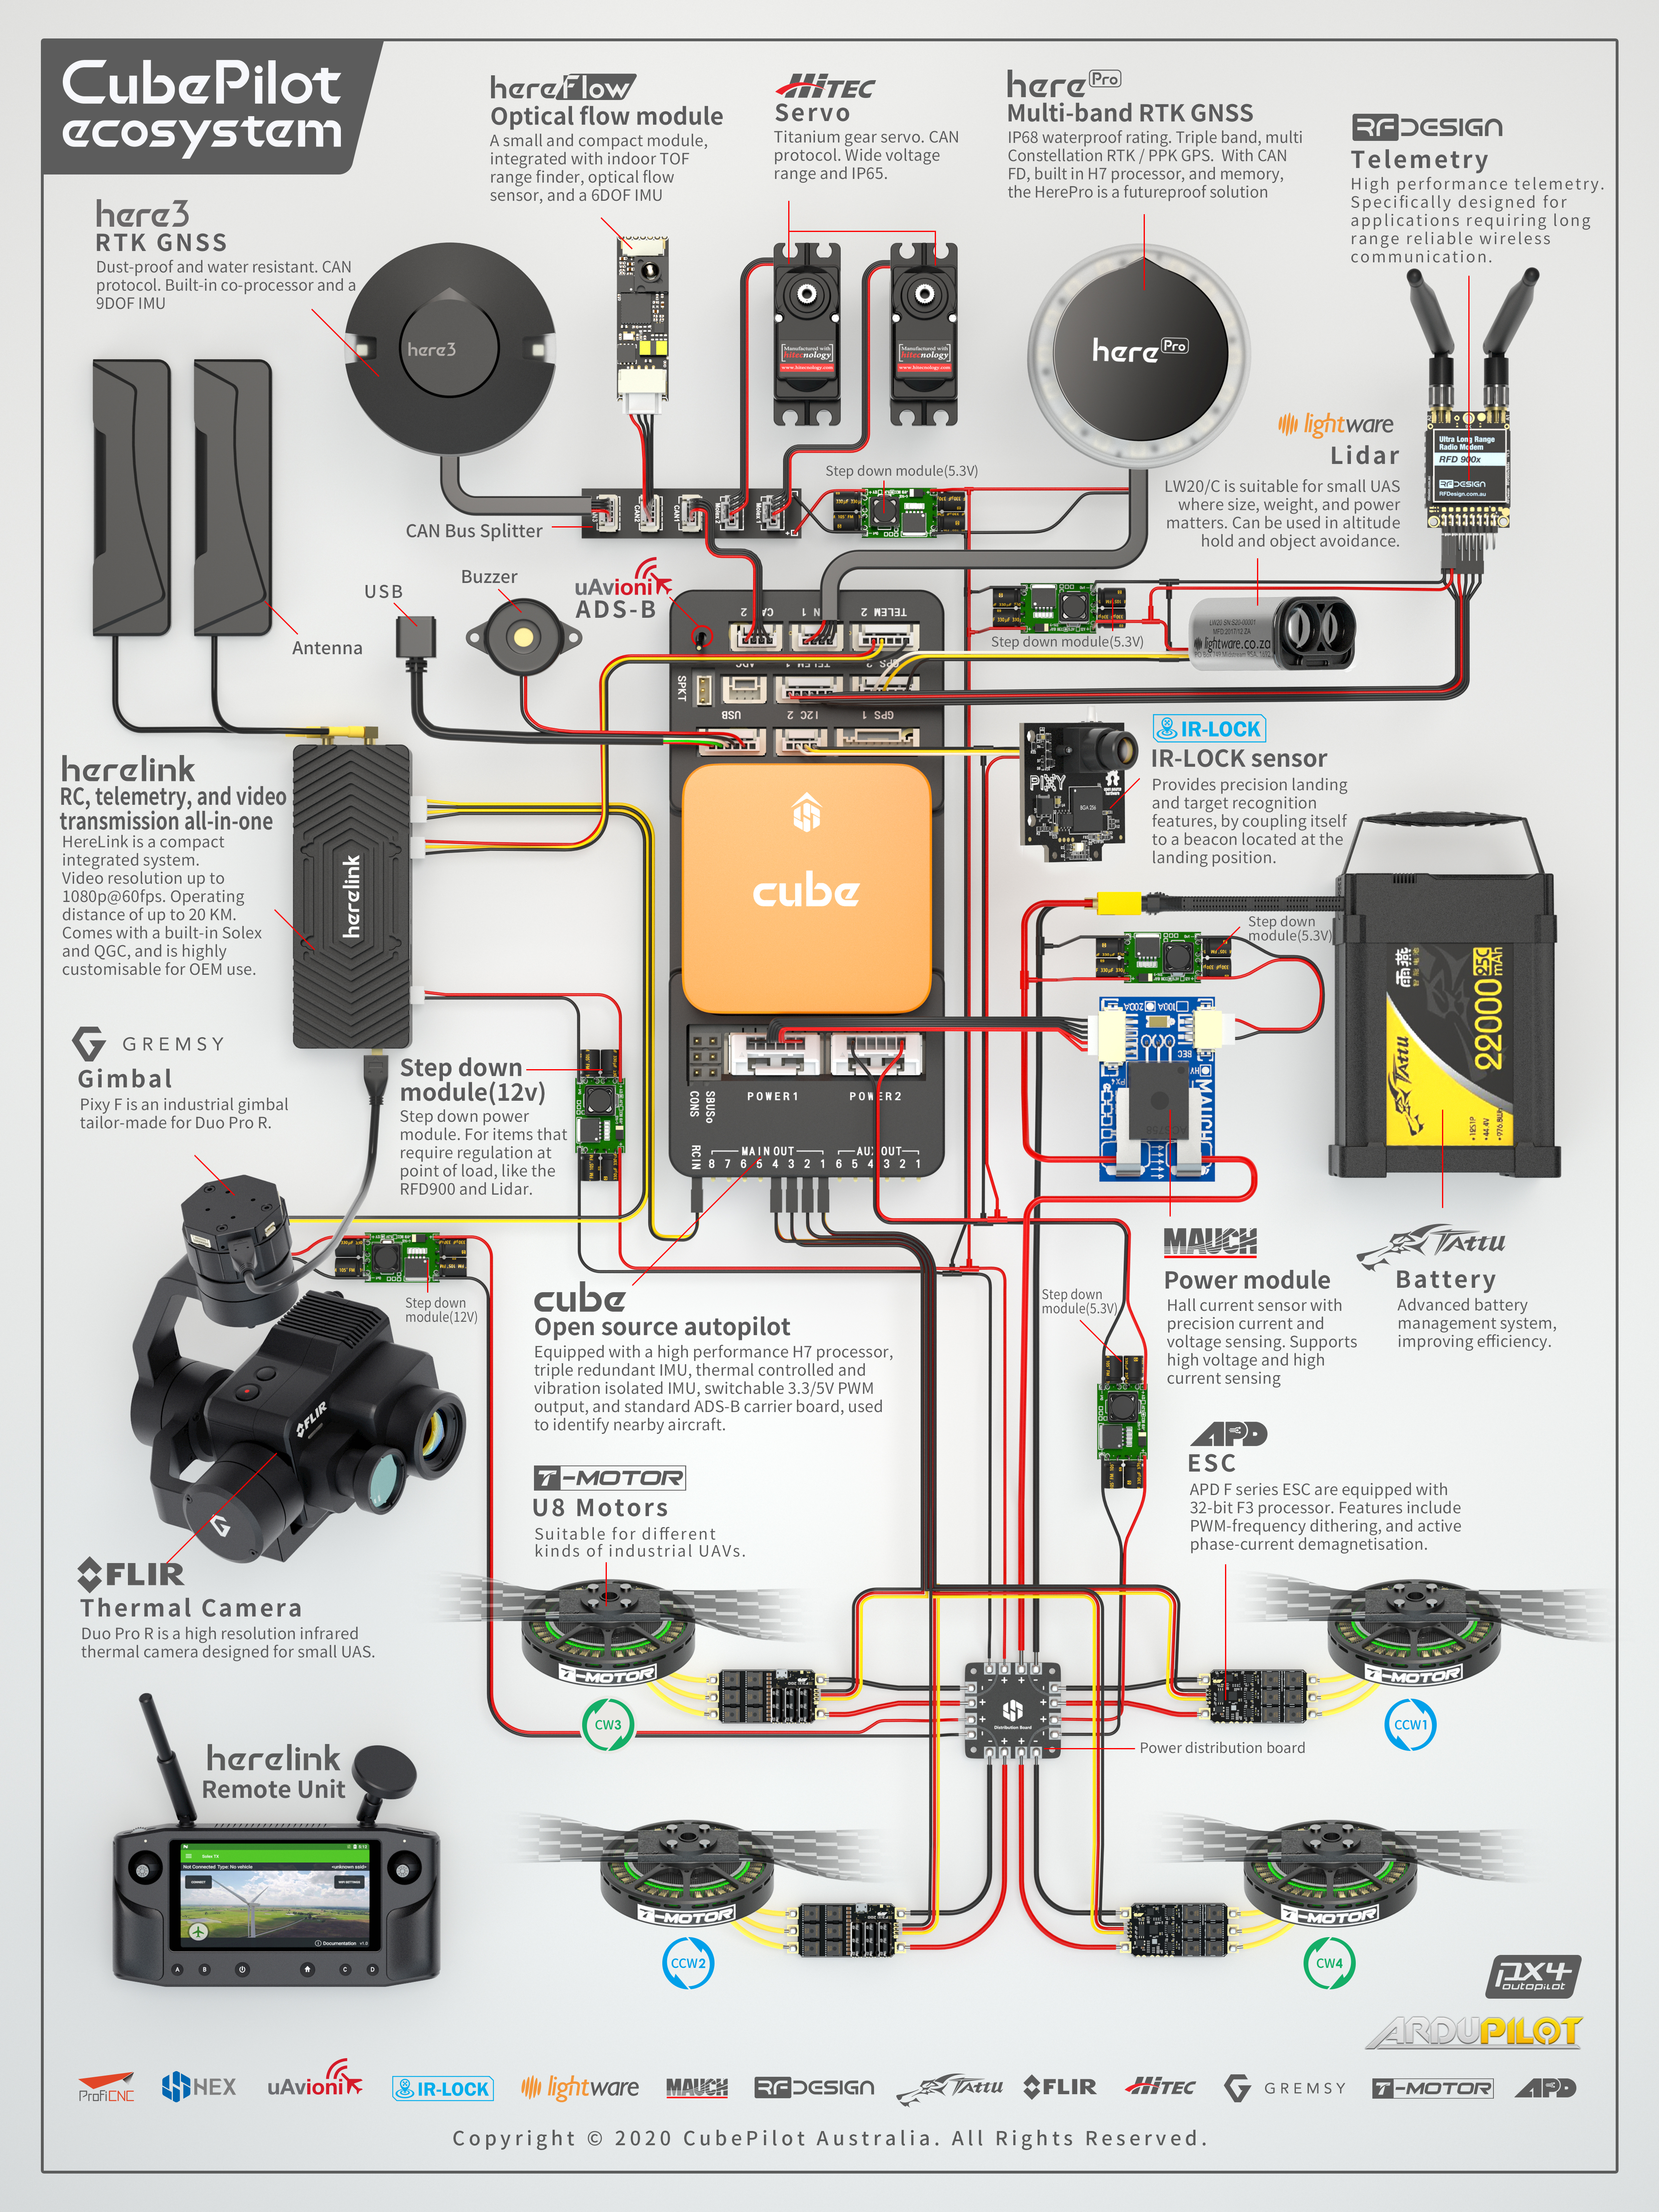
\includegraphics[width=0.4\textwidth]{images/cubepilot-ecosystem.jpg}
    \caption{The Cubepilot Ecosystem\cite{ardupilot}}
    \label{fig:cubepilot-ecosystem}
\end{figure}
The Hex Cube Black is an ArduPilot compatible autopilot.
\section{ArduCopter}
The firmware that the Pixhawk runs is the Arducopter, the copter specific version of ArduPilot, it is an open source firmware that supports the fully autonomous waypoint based flight and real time control, using MAVLink protocol to communicate with the Remote \gls{gcs}. The \gls{gcs} software used is Mission Planner.
\section{Mission Planner}
Mission Planner is a full-featured ground station application for the ArduPilot open source autopilot project \cite{ardupilot}.
It is used to configure the vehicle and plan the missions.
\begin{figure}[H]
    \centering
    \includegraphics[width=0.7\textwidth]{images/mission-planner.PNG}
    \caption{Screenshot of Mission Planner main screen, the gps is fixed in the laboratory location and the telemetry data is shown.}
    \label{fig:mission-planner}
\end{figure}
